\chapter{Experimental Evaluation}

\noindent For the purposes of evaluating Modulo7, test cases have been designed into two formats. One category of testing is micro testing, for validating correctness and precision recall for small sets of data. This ensures verifiability of algorithms and similarity measures on small datasets as well as novel explorations of data. Most MIR research is done on small scale datasets and hence falls in the purview of micro testing. The other format is macro testing which involves large datasets such as the million song dataset \cite{msd}. \\\\
A few assumptions that are made in testing are as follows :-
\begin{enumerate}
\item In order to estimate ground truth values, the author assumed ground truth values presented in datasets used / or subjective judgments about which songs are similar to each other. These subjective judgments are procured from existing literature.
\item If the song meta data (such as key-signature, time-signature, total duration of song) is not encoded, its estimated by the individual parsers for the data source. This estimation id done by existing algorithms in literature. However if meta data is encoded in the input, its assumed to be correct and no such estimations are carried out. 
\item Most tests are against file formats of the similar types (for example midi is tested against other symbolic files). This is due to the inherent complexity of symbolic decoding of audio formats like mp3. Also its easier to compare symbolic data against other symbolic data.
\item In the event of parsing data, there can be legal issues (e.g. the song can be copyrighted). For that reason custom parsers to build alternate research datasets (e.g the million song dataset has already derived features that Modulo7 intended to derive for Mp3 files and has its own parser written by the authors. \cite{msd})
\item All evaluations are done against research datasets which are published in academia or exposed as public data sets in industry. As such no proprietary data sets are used for the purpose of any evaluation metric.
\end{enumerate}

\section{Results of Index Compression}

\noindent The Modulo7 representation can be thought of an indexed meta data version of the song with the symbolic information of the song intact. True to all indexed data, Modulo7 represents the song in a much smaller size than the original source. The following chart demonstrates the average compression of indexed data as compared to source files on the Saarland Music Data (SMD) Dataset \cite{saarlandmsd}:-
\begin{figure}
\centering
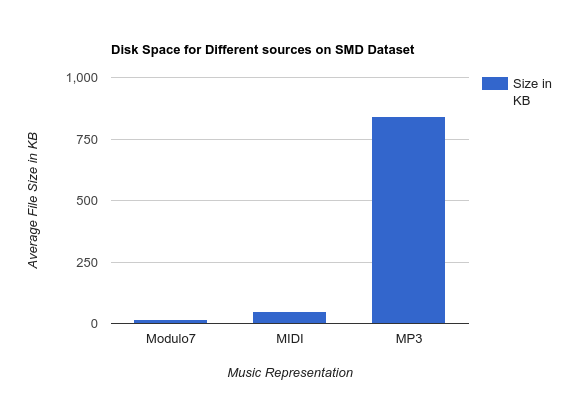
\includegraphics[width=\textwidth]{Modulo7SMDBarGraph.png}
\makeatletter
\let\@currsize\normalsize
\caption{Modulo7 architectural design}
\label{fig:figure}
\end{figure}
As expected Modulo7's serialized format expresses a song in less disk space than its source formats while keeping the symbolic information intact. The results are positive as there is a 4 time decrease in size of expressing symbolic information as compared to midi files. \\\\
A similar transformation was also done on a direct download able subset of the wikifonia dataset in order to compare Modulo7 internal representation against the compressed xml representation of the wikifonia dataset. A plot of disk space requirements are plotted in ascending order of the wikifonia dataset file sizes:- 
\begin{figure}
\centering
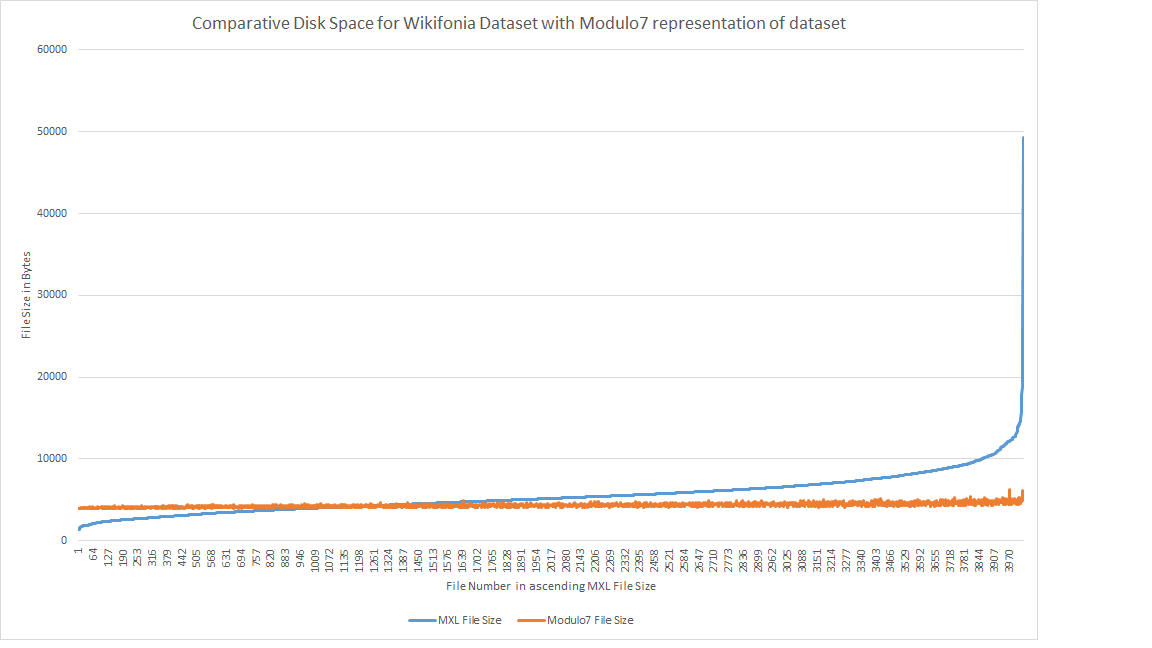
\includegraphics[width=\textwidth]{M7Graph.png}
\makeatletter
\let\@currsize\normalsize
\caption{Modulo7 comparative file sizes}
\label{fig:figure}
\end{figure}

\noindent As expected, Modulo7 is extremely space efficient for storing symbolic information.
\section{Results on similarity measures}

\noindent This set of experiments determine the precision and recall values for the similarities defined in \ref{similarity} on ground truth data extracted from \cite{msd}. Modulo7 does not claim to improve on the state of the art when it comes to similarity metrics or does not intend to create a new similarity metric. Rather this set of experiments are a test of efficiency in execution and accuracy of existing methods on large scale datasets. The million song dataset was chosen for experimental evaluation \cite{msd} for pre computed symbolic transcriptions of mp3 data and the last fm data set for ascertaining similar songs to build a ground truth for evaluation. Due to the constraints of hardware for evaluation, we took a scaled down subset of the original 584,897 songs to a more manageable 10000 songs, with similar songs edited to fit this dataset. The songs were chosen randomly from the dataset with the only criteria being that they are monophonic(since polyphonic transcription from audio files is not a fully solved problem \cite{melextract}). As a consequence only the monophonic similarity measures are used for these experiments. 

\section{Results on KK Tonality Profiles algorithm}

\noindent In order to test the KK Tonality algorithm given in \ref{kktonality}, Modulo7 is benchmarked against a big subset of the Wikifonia data set of lead sheets in the compact mxl format (variant of the music xml format) \cite{WikifoniaDataset}. The original dataset of the Wikifonia is now no longer available but a sizable subset of 6715 songs are currently down loadable and copyright free. Out of this set, 1314 have key signatures embedded in the song sources. The experiment involves comparing the key signatures embedded inside the key signatures versus the implied key signatures the KK Tonality estimates from the pitch histogram of the songs parsed from this source. A special MXL parser (a minor variant of the music xml parser) was developed for this purpose. The scoring scheme for this experiment was simple, if the key signature was correctly identified then score of 1 otherwise score of 0. In this particular dataset, key signatures are partially known (\textbf{since the number of sharps or flats in the key signatures are always encoded in music xml files} so only relative major/minor are needed to be ascertained). As a consequence only two choices are to be made between key signatures for each file giving a baseline of 50 percent. In this particular example, KK Tonality's performance is how well it can distinguish between relative minors and majors. \\\\
After running the KK Tonality algorithm on the wikifonia dataset, 1129 out the total 1314 key signatures are correctly identified leading to an accuracy of \text{85.9 percent}. This is commensurate with the reported accuracies in \cite{kkTonalityKeyFinding}. The novelty of this experiment stems from the fact that KKTonality profiles algorithm was not successfully run against a large scale database successfully in literature. 

\section{Results on lyrics similarity and statistics analysis}

\noindent On top of the experiments done for Song sources incorporating tonal information, there were specific experiments that were carried out for lyrics similarities in general. The ground truth for these experiments is the musix match lyrics dataset present in the million song data set \cite{msd}. The dataset decomposes lyrics into bag of words formats (the frequencies of the top 5000 words in lyrics) along with bag of words representation of 210,519 lyrics of songs. This dataset acts like a great baseline for set based similarities of lyrics. The experiment involved calculating the expected word count from the ground truth data and with that form a basis for comparing songs with the ground truth data. There are measures defined in literature \cite{lyricsRanking} which define similarity and accuracy of lyrics based on expected counts of words and observed counts of words in lyrics. However for this experiment we have decided to extract the tags from the last fm dataset of the Million Song Data set \cite{msd} to acquire the tags that occur frequently for a given song and then build a predictive model that outputs the tags for a newly seen song. \\\\
These tags could indicate the language, genre etc of the songs. As such this comparison allows for predicting various meta data regarding a newly seen lyrics of a song and allow for building a model that predicts tags based on lyrics similarities. \\\\
Out of the 210,519 songs with lyrics provided in the million song data set, 2296 have tags extracted for them in the dataset, so this set of songs are considered the ground truth for estimating tags for novel lyrics. The lyrics in this dataset are in the bag of words document representation format and hence standard similarity measures like cosine and dice similarity can be used for similarity measurement between lyrics. The lyrics in the million song dataset are already stemmed via the Porter stemmer \cite{msd} \\\\
In order to estimate the accuracy of the tag prediction models, the extracted data was divided into 10 percent test data and 90 percent training data and 10 fold cross validation was performed. Each lyrics in the test data was compared to the training data and a ranked order of the trained songs are presented based on the similarity metric used. Tags are then estimated based on the tag estimation mechanisms presented in \ref{lyricsarch}. The similarity metrics for comparing lyrics that were chosen for this experiment were standard document similarity measures that are word transpose invariant (cosine similarity, dice similarity etc). In order to estimate the degree of agreement of the estimated tag set with the observed tag set for a given song, we use the Jaccard Similarity which is defined as 
\begin{equation}
J(T_{est}, T_{obs}) = \frac{\mid T_{est} \cap T_{obs} \mid}{\mid T_{est} \cup T_{obs} \mid}
\end{equation}
The following table lists out the observed average agreement over all songs of the test set:-\\

\begin{tabular}{ |p{4cm}||p{3cm}|p{3cm}|p{3cm}|  }
 \hline
 \multicolumn{4}{|c|}{Precision and recall values based for lyrics estimation schemes} \\
 \hline
 Estimation Scheme     or Area Name& ISO ALPHA 2 Code &ISO ALPHA 3 Code&ISO numeric Code\\
 \hline
 Naive Estimation   & AF    &AFG&   004\\
 Weighted Estimation &   AX  & ALA   &248\\
 Albania &AL & ALB&  008\\
 \hline 
\end{tabular}

\section{Result on Memory and Disk space usage against jMIR}

\noindent In order to compare the memory and disk space requirements, Modulo7 was tested against its closest competitor jMIR's \cite{jMIR} jSymbolic component. Both frameworks are written in Java and both involve extraction of features(although that is not an end goal for Modulo7). However jMIR is more exhaustive in what features it extracts so only a subset of those that are also extracted by Modulo7 are considered. Out of the total 111 features that are implemented in jSymbolic \cite{jSymbolic}, 23 features were identified as implemented as internal computation within the Modulo7 indexers and/or querying engine. \textbf{Its important to note that unlike jMIR, Modulo7 is not an exhaustive feature extractor}. The features identified  
\begin{enumerate}
\item 1 feature for duration of song
\item 2 features for average melodic intervals, note duration
\item 1 feature for Meter classification (simple or compound)
\item 1 feature for lengths of melodic archs in midi files
\item 1 feature for initial tempo of song
\item 4 features for melodic intervals (thirds, fifths, octaves and intervals in the bass line)
\item 2 features for maximum and minimum durations of notes in the song
\item 3 features for most commonly occurring pitch, pitch class and melodic interval
\item 3 features for ranges, namely primary register, range of highest and lowest voices
\item 1 feature for time signature
\item 4 features for checking for voice equality in the following categories : melodic leaps, note duration, number of notes and range
\end{enumerate}
\noindent In order to compare the frameworks, the author used jProfiler to profile for average CPU and Memory usage and time taken for both frameworks over different sized subsets of the Saarland Music Data (SMD) Dataset \cite{saarlandmsd}. In order to protect against background process interference, the frameworks were ran on AWS EC2 m4x.large instances (dual core 2.4 GHz Intel Xeon® E5-2676 v3 (Haswell) processors
and 8 GB DDR3 RAM). We plot the average memory consumed, CPU load and time taken in seconds as a function of dataset size (over monotonically increasing subset sizes of the SMD dataset). We ignore IO performance since in this experiment, IO is only utilized when pushing output to disk, which is not taken as a metric of evaluation. No data sets involving music xml files were chosen, as jSymbolic does not support music xml files. 
The plot for time taken (in seconds) for both jSymbolic and Modulo7 is plotted as a function of dataset size :-


